\documentclass[11pt]{article}
\usepackage{amsmath}
\usepackage{amsfonts}
\usepackage{listings}
\usepackage{graphicx}
\usepackage{xcolor}

\newcommand{\numpy}{{\tt numpy}}    % tt font for numpy

\topmargin -.5in
\textheight 9in
\oddsidemargin -.25in
\evensidemargin -.25in
\textwidth 7in

\begin{document}

% ========== Edit your name here
\author{Shiyu Li \\ shiyu.li@duke.edu}
\title{Lab 2: Construct, Train, and Optimize Neural Network Models}
\maketitle

\medskip

% ========== Begin answering questions here
\begin{enumerate}

\item
Assignment 1

We can do this calculation layer by layer:

\begin{enumerate}
    \item C1 (Layer 1)
        MAC = $28\times 28 \times 3 \times 5 \times 5 \times 6 = 352800$ 
        Params = $5\times 5\times 3 \times 6 + 6  = 456$
    \item C2 (Layer 3)
        MAC = $10\times 10 \times 6 \times 5 \times 5 \times 16 = 240000$
        Params = $6\times 5 \times 5 \times 16 + 16 = 2416$
    \item FC1 (Layer 5)
        MAC = $5\times 5\times 16 \times 120 = 48000$
        Params = $5\times 5\times 16 \times 120 + 120 = 48120$
        
    \item FC2 (Layer 6)
        MAC = $120 \times 84 = 10080$
        Params = $120*84 + 84 = 10164$
        
    \item FC3 (Layer 7)
        MAC = $84 \times 10 = 840$
        Params = $84 * 10 + 10 = 850$
        
\end{enumerate}

In total, we have $MAC = 651720 = 6.5M, Params= 62006$

\item
Assignment 2

The code can be found on https://github.com/timlee0212/ECE590.10-Lab2

Note: The version on the repo is the finetuned version but also meet the requirement of the assignment 2.

\item
Assignment 3

\begin{enumerate}
    \item Initial loss (the evaluation before training) is $2.3052$
    
    When I tried to reach 65\% validation accuracy as said in assignment, I found it varies for different runs, as shown in Fig.\ref{fig:var_init}. The reason might be the initialization of the weight. Since we do not set the random seed of each run, the initial point is different, which will lead to different result of the optimization.
    
    From the learning curve we can also see that after around 10 epochs, the network was overfitting. Though the training loss is on decreasing and the training accuracy is on increasing, the validation loss is increasing and the validation accuracy is decreasing. The network 'learned' too much information about the training set. 
    \begin{figure}[h]
        \centering
        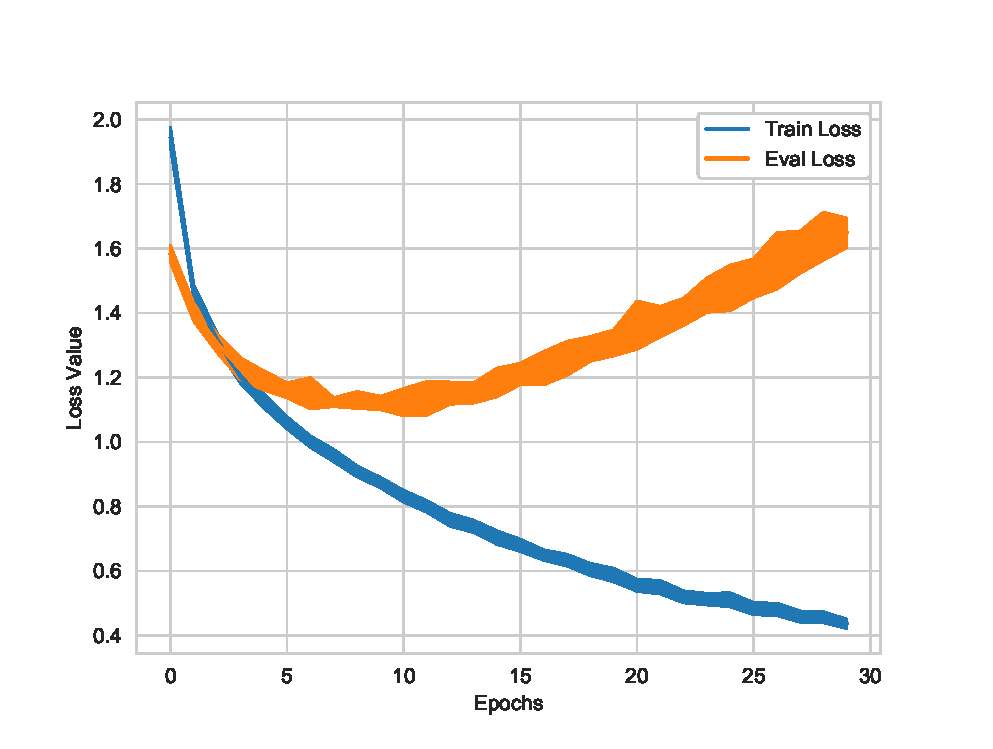
\includegraphics[width=0.45\linewidth]{initial_train_var_loss.eps}
        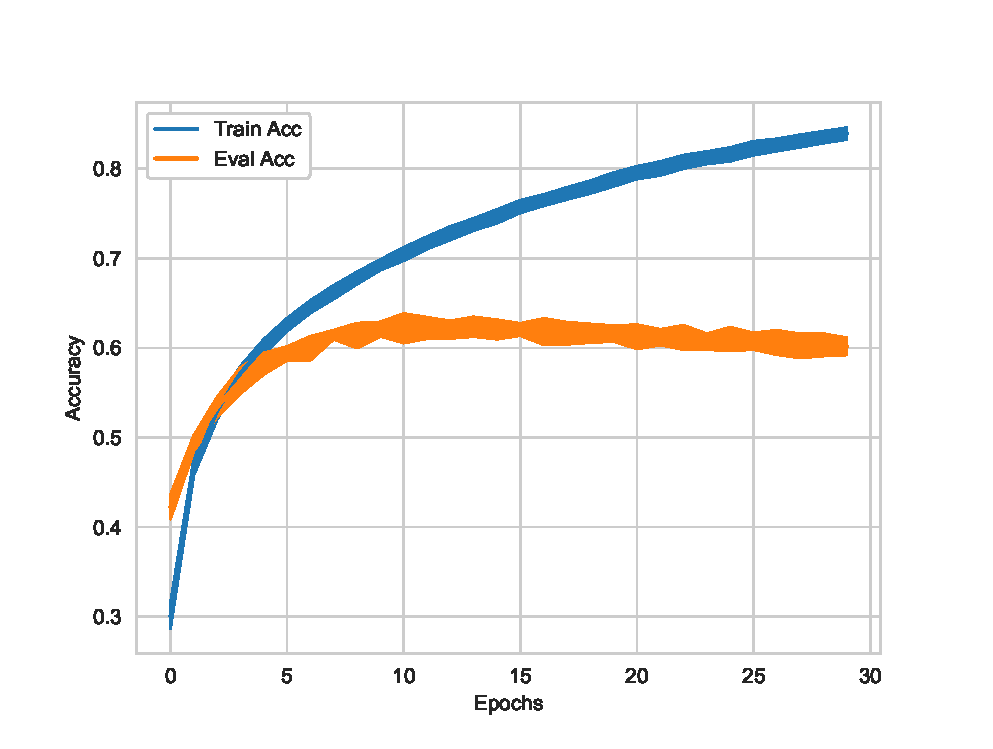
\includegraphics[width=0.45\linewidth]{initial_training_var_acc.eps}
        \caption{The accuracy and loss curve of the initial training settings of 10 runs.}
        \label{fig:var_init}
    \end{figure}
    
    \item In addition to \textit{ToTensor} and \textit{Normalize}, I added random flip and random crop as the data augmentation method. The comparison of learning curve is shown as Fig.\ref{fig:data_aug}. From the curve we can see that with data augmentation enabled, the training accuracy is much lower while the training loss decreases much slower. However, the validation accuracy is higher and the validation loss continues to decrease as the training process going. No overfitting happened and the training accuracy and loss is very close to the validation ones.
    
    Data augmentation can been seen as enlarging the training set. Although it may seems to make the training process slower, it prevent the network from overfitting the training set and boost the generalization ability of the neural network. 
    
    \begin{figure}[h]
        \centering
        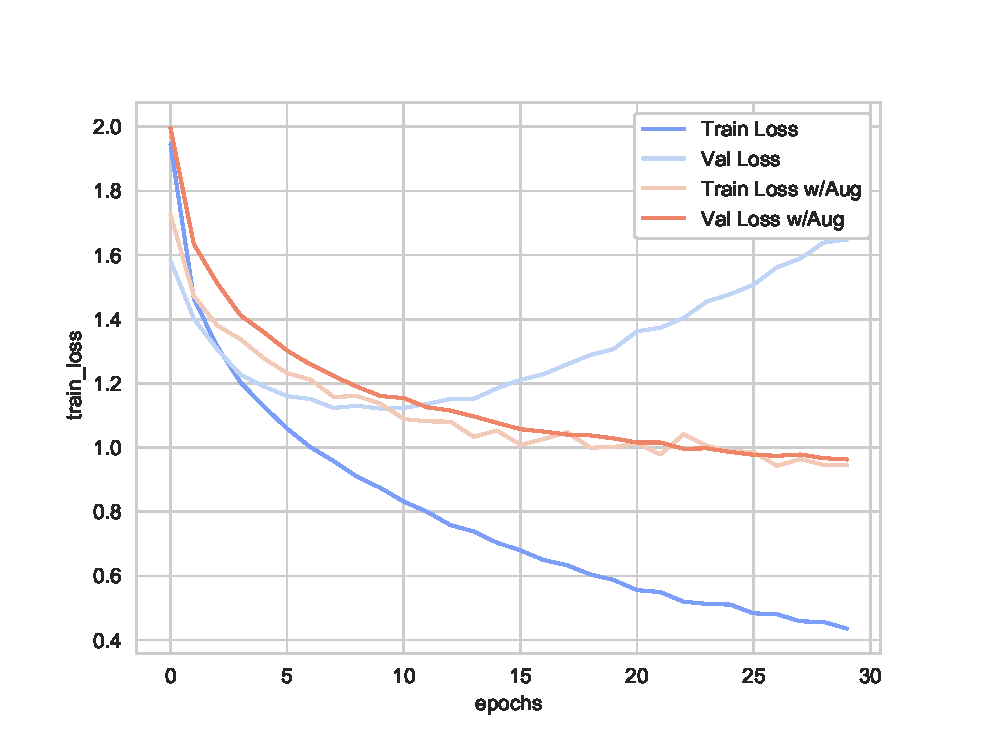
\includegraphics[width=0.45\linewidth]{data_agu_loss.eps}
        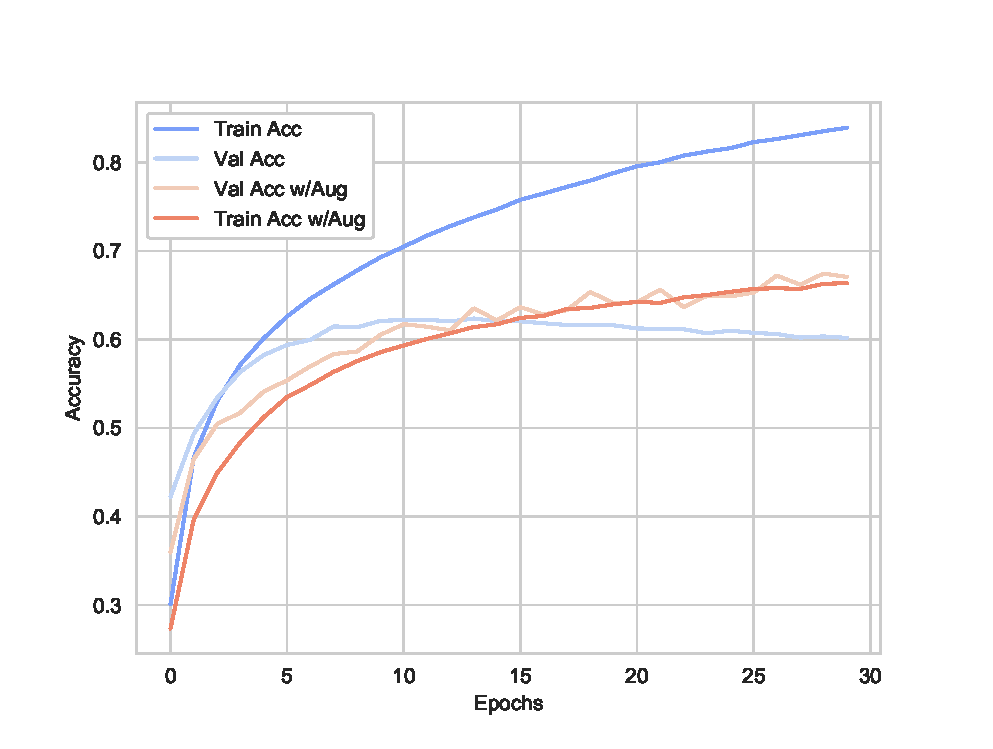
\includegraphics[width=0.45\linewidth]{data_agu_acc.eps}
        \caption{The accuracy and loss curve of data augmentation enabled compared to initial setting.}
        \label{fig:data_aug}
    \end{figure}
    
    \item 
    
    \begin{figure}[h]
        \centering
        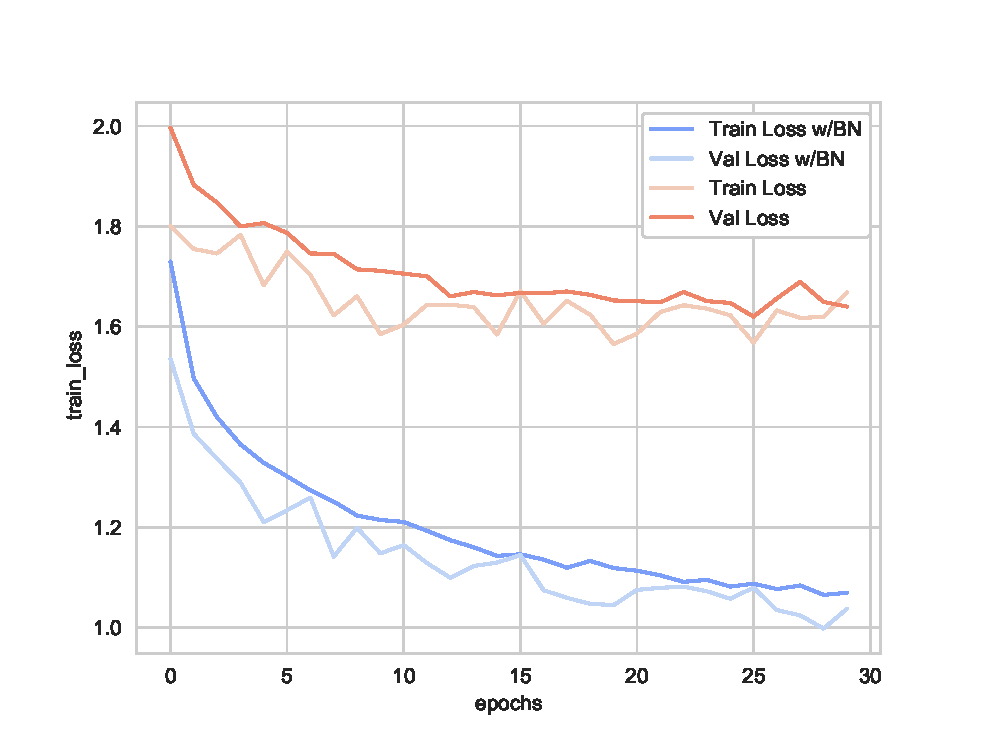
\includegraphics[width=0.45\linewidth]{BN_LR01_Loss.eps}
        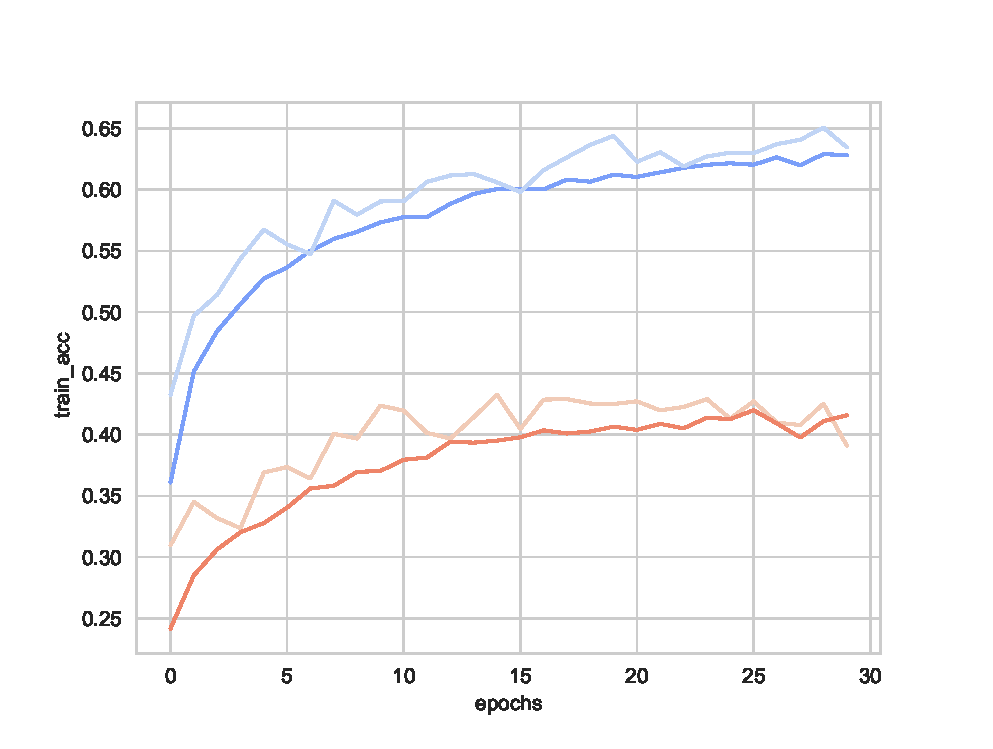
\includegraphics[width=0.45\linewidth]{BN_LR01_Acc.eps}
        \caption{The accuracy and loss curve of Batch Normalization inserted compared to initial setting, with learning rate set to 0.1.}
        \label{fig:my_label}
    \end{figure}
\end{enumerate}

\end{enumerate}

\end{document}
\grid
\grid